\documentclass[12pt]{article}
\usepackage[utf8]{inputenc}
\usepackage{graphicx}
%opening
%\title{Estudio de estrellas de Plank OJO}
%
%\author{
%	\Large Alejandro Hernández A.\\
%	\large 201219580
%	    }
%\date{\vspace{-5ex}}
%\date{Noviembre 6, 2015.}
%
%\setlength{\parindent}{0pt}
%\renewcommand{\indent}{\hspace*{\tindent}}

\begin{document}

%\maketitle
\begin{center}
\Huge
Estudio de estrellas de Plank OJO

\vspace{3mm}
\Large Alejandro Hernández A.

\large
201219580


\vspace{2mm}
\Large
Director: Pedro Bargueño de Retes

\normalsize
\vspace{2mm}

\date{Noviembre 6, 2015.}
\date
\end{center}



\section{Protoboard}

Un protoboard es un tablero con orificios conectados internamente mediante cables eléctricos, que permite insertar componentes electrónicos tales como resistencias, condensadores e inductores para armar circuitos eléctricos.
\\

Internamente, un protoboard se compone por bloques de plástico perforados y de diversas láminas delgadas (aleación de cobre, estaño y fósforo) que unen las mencionadas perforaciones, creando así líneas de conducción paralelas. Las líneas se cortan en la parte central del bloque para permitir que dispositivos en circuitos integrados puedan ser insertados perpendicularmente, sin ser tocados por los experimentadores, a las líneas de conductores. En la cara opuesta se coloca un forro que sella y mantiene fijas las tiras metálicas.
\\

La estructura externa de un protoboard se muestra a continuación:
\\

\begin{figure}[h!]
	\centering
	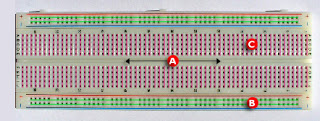
\includegraphics[width=0.6\textwidth]{protoboard}
	\caption{Protoboard.}
\end{figure}

Donde:

\begin{itemize}
	\item \textbf{Canal Central:} Usado para colocar los circuitos integrados. 
	\item \textbf{Buses:} Usados para conectar la fuente de voltaje.
	\item \textbf{Pistas:} Aquí se conectan resistencias, conductores, inductores, entre otros elementos electrónicos.

\end{itemize}

\section{Conexiones en serie y en paralelo}

A continuación se ilustran las distintas formas de conectar resistencias en una protoboard.
\\

\begin{figure}[h!]
	\centering
	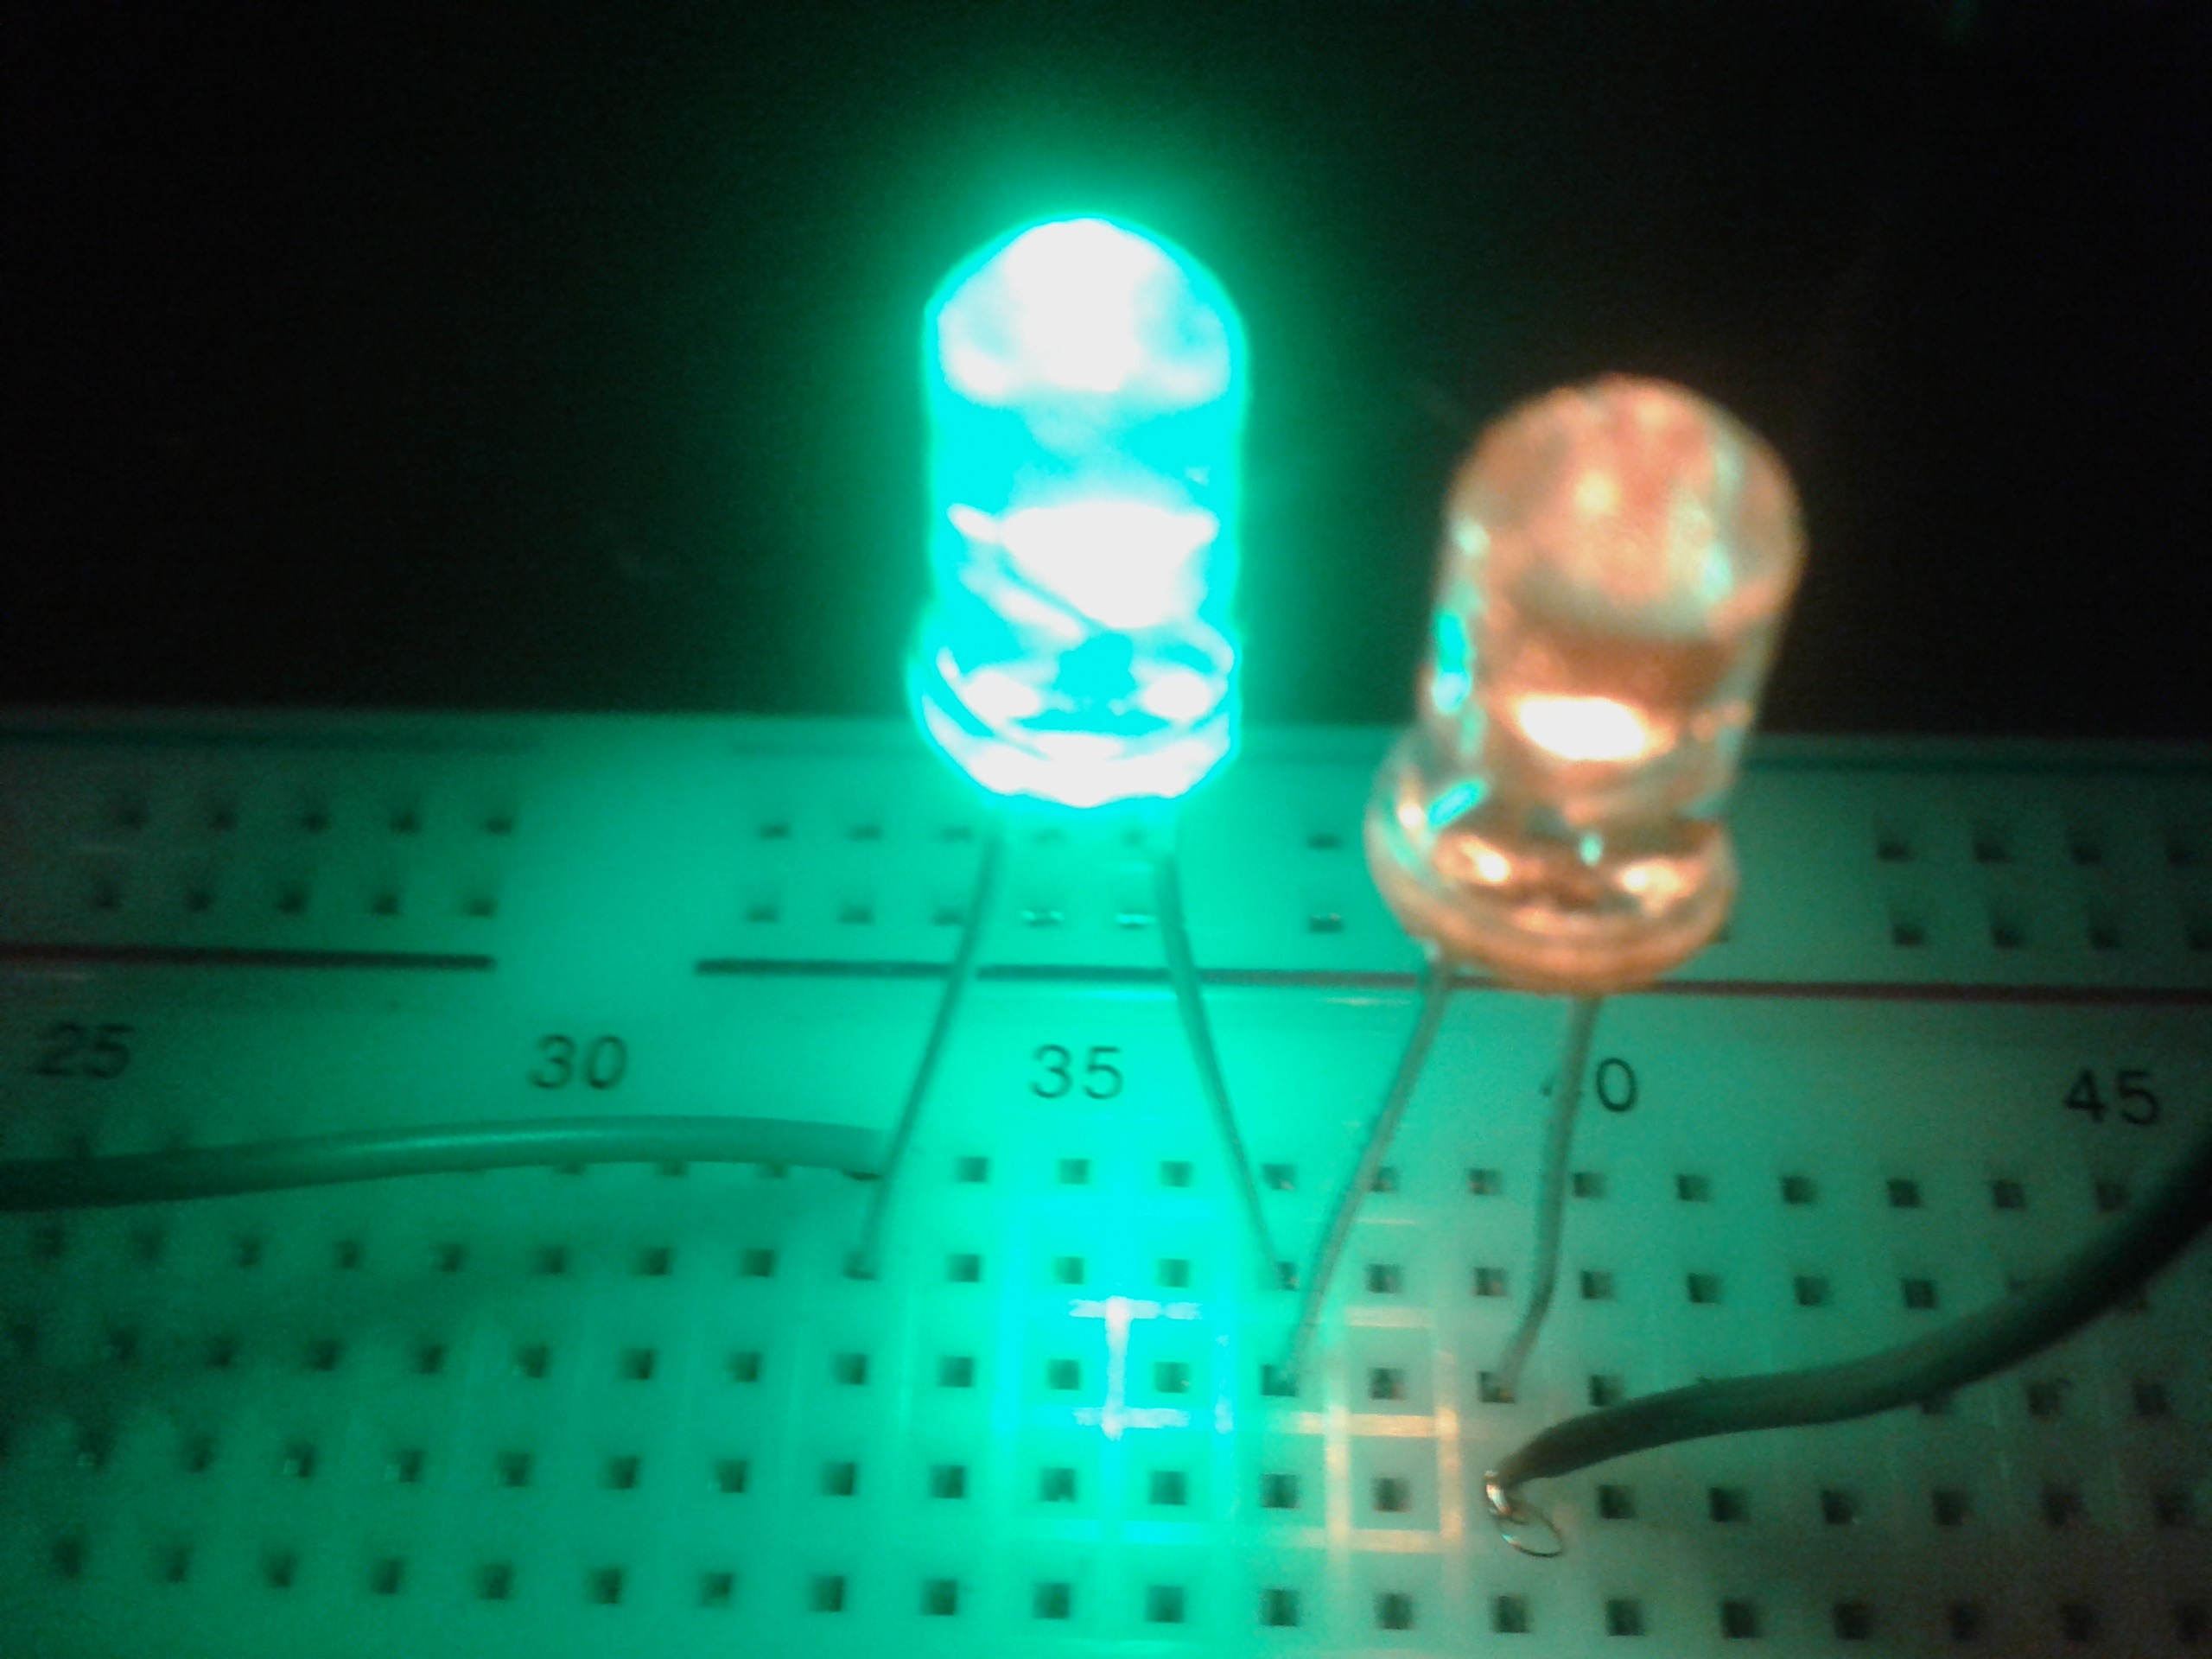
\includegraphics[width=0.4\textwidth,height=0.17\textheight]{serie}
	\caption{Resistencias conectadas en serie.}
\end{figure}

\begin{figure}[h!]
	\centering
	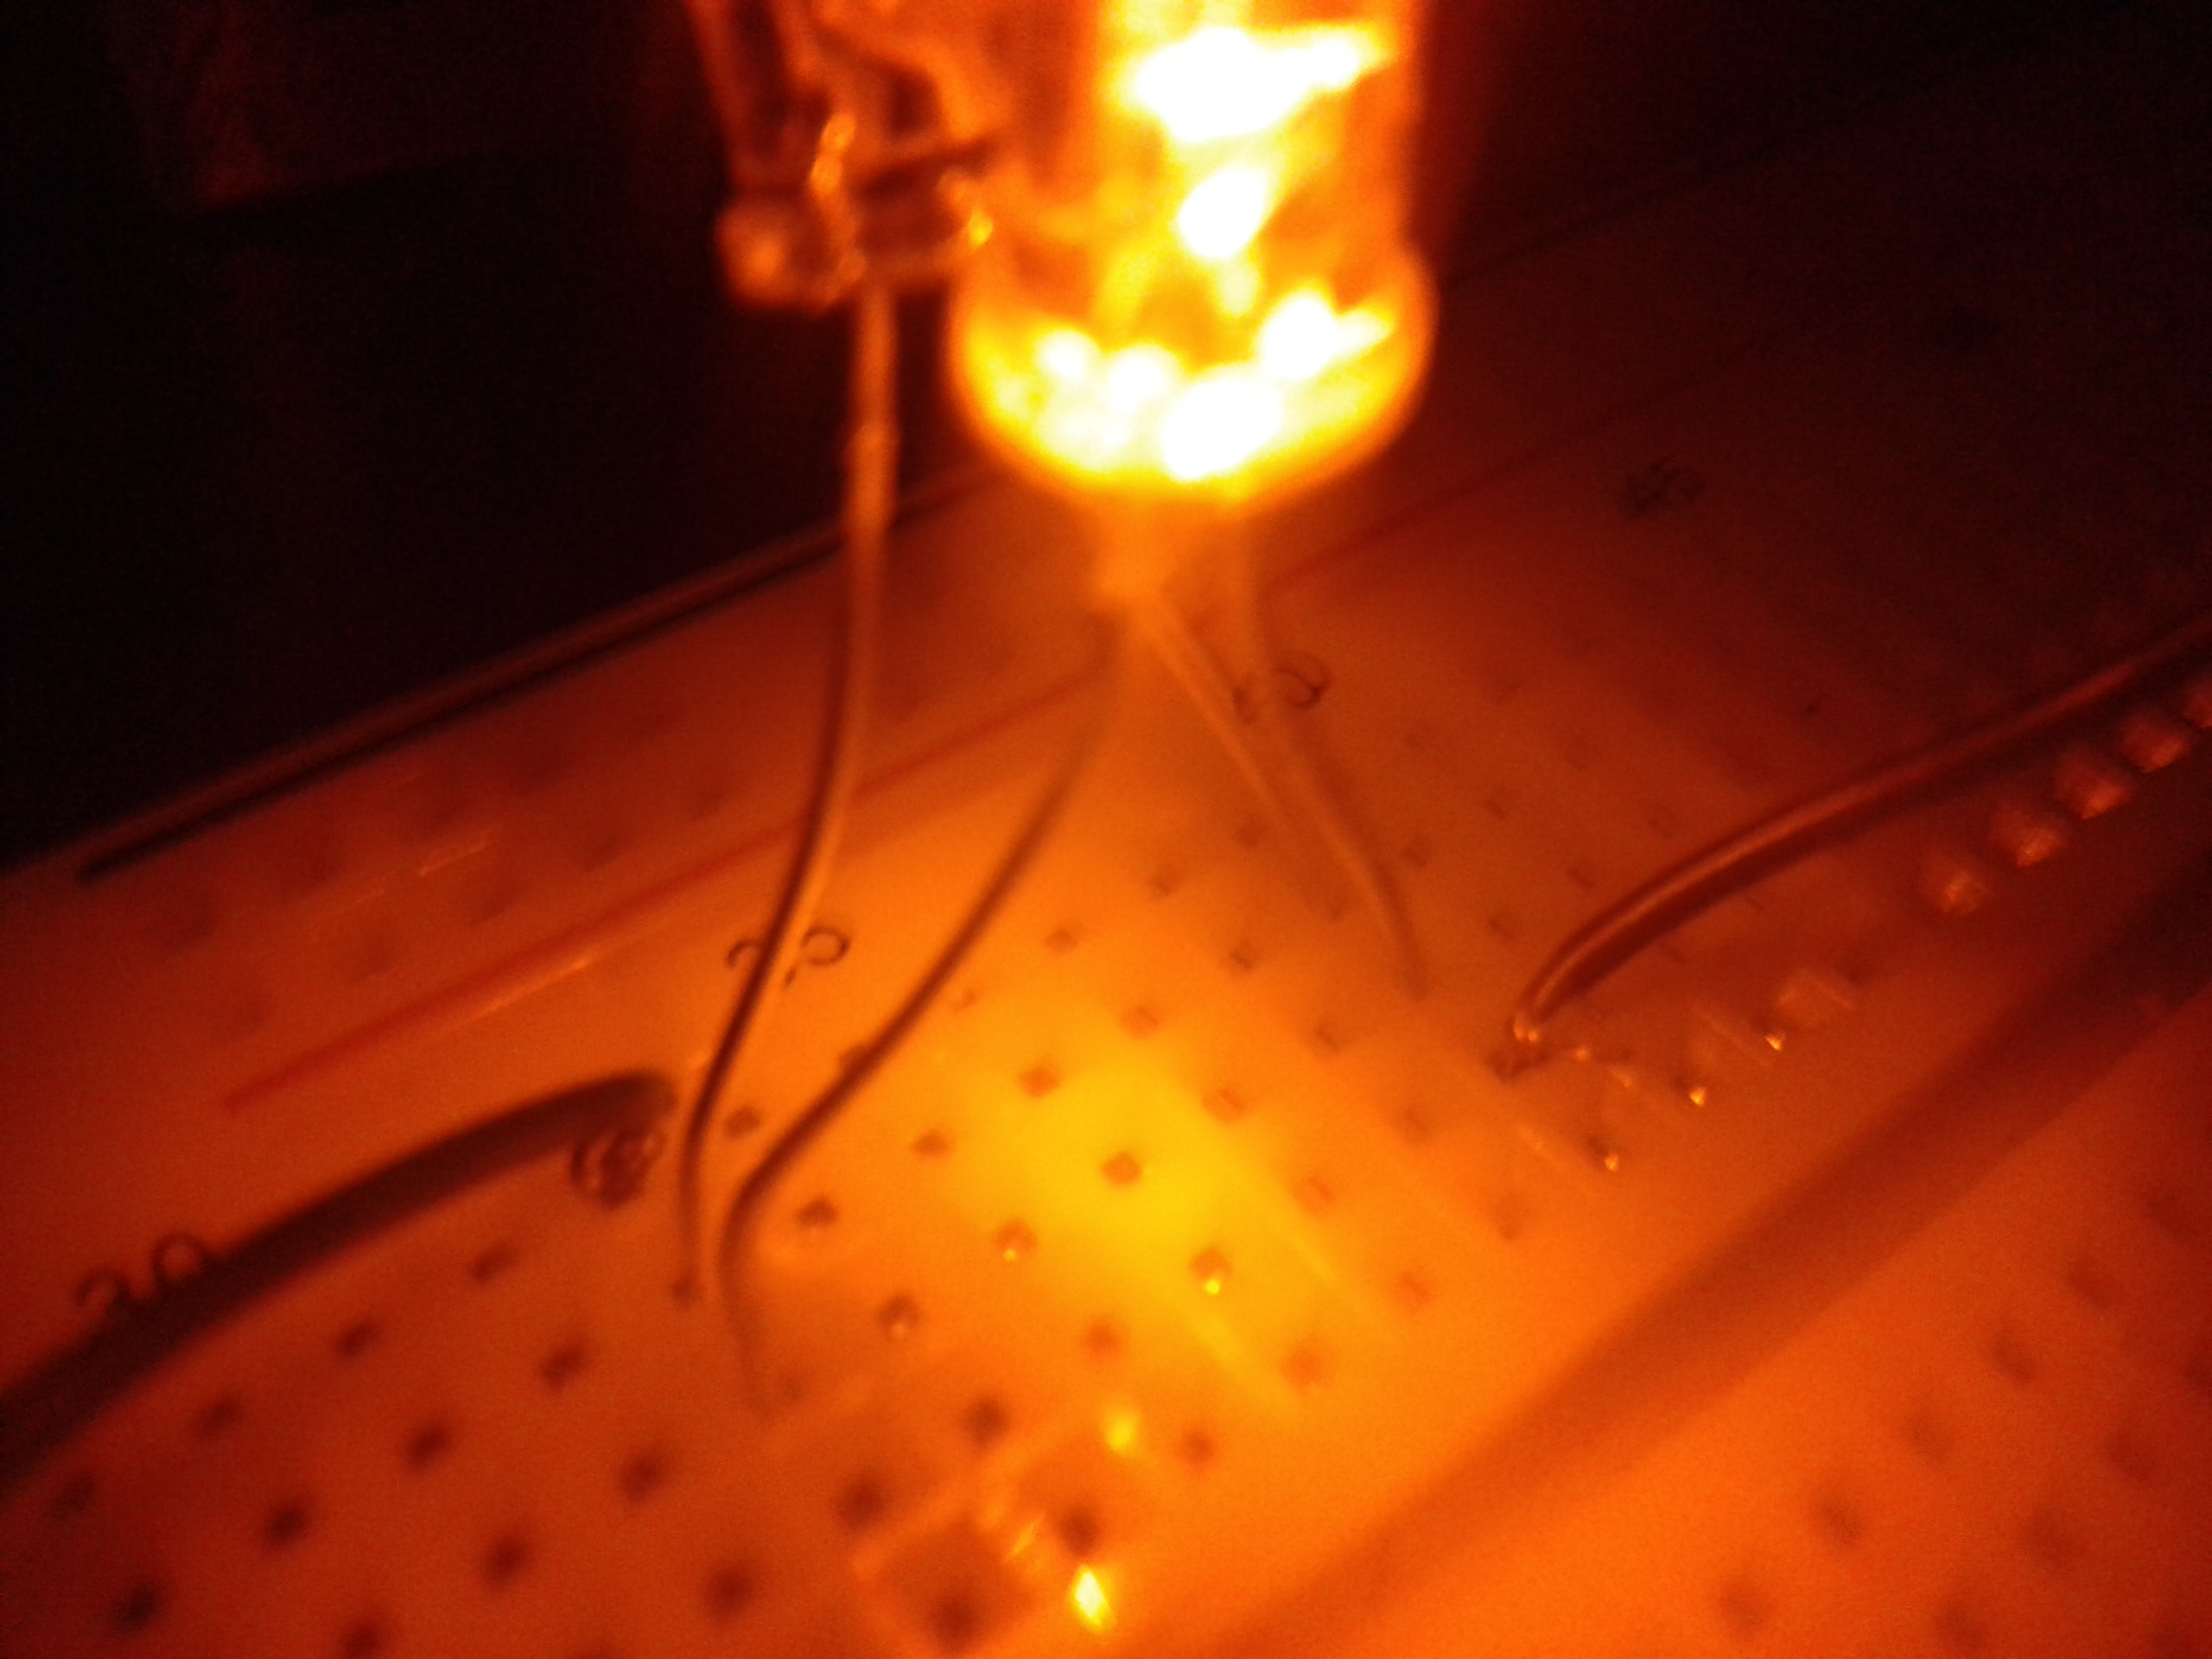
\includegraphics[width=0.4\textwidth,height=0.17\textheight]{paralelo}
	\caption{Resistencias conectadas en paralelo.}
\end{figure}

\begin{figure}[h!]
	\centering
	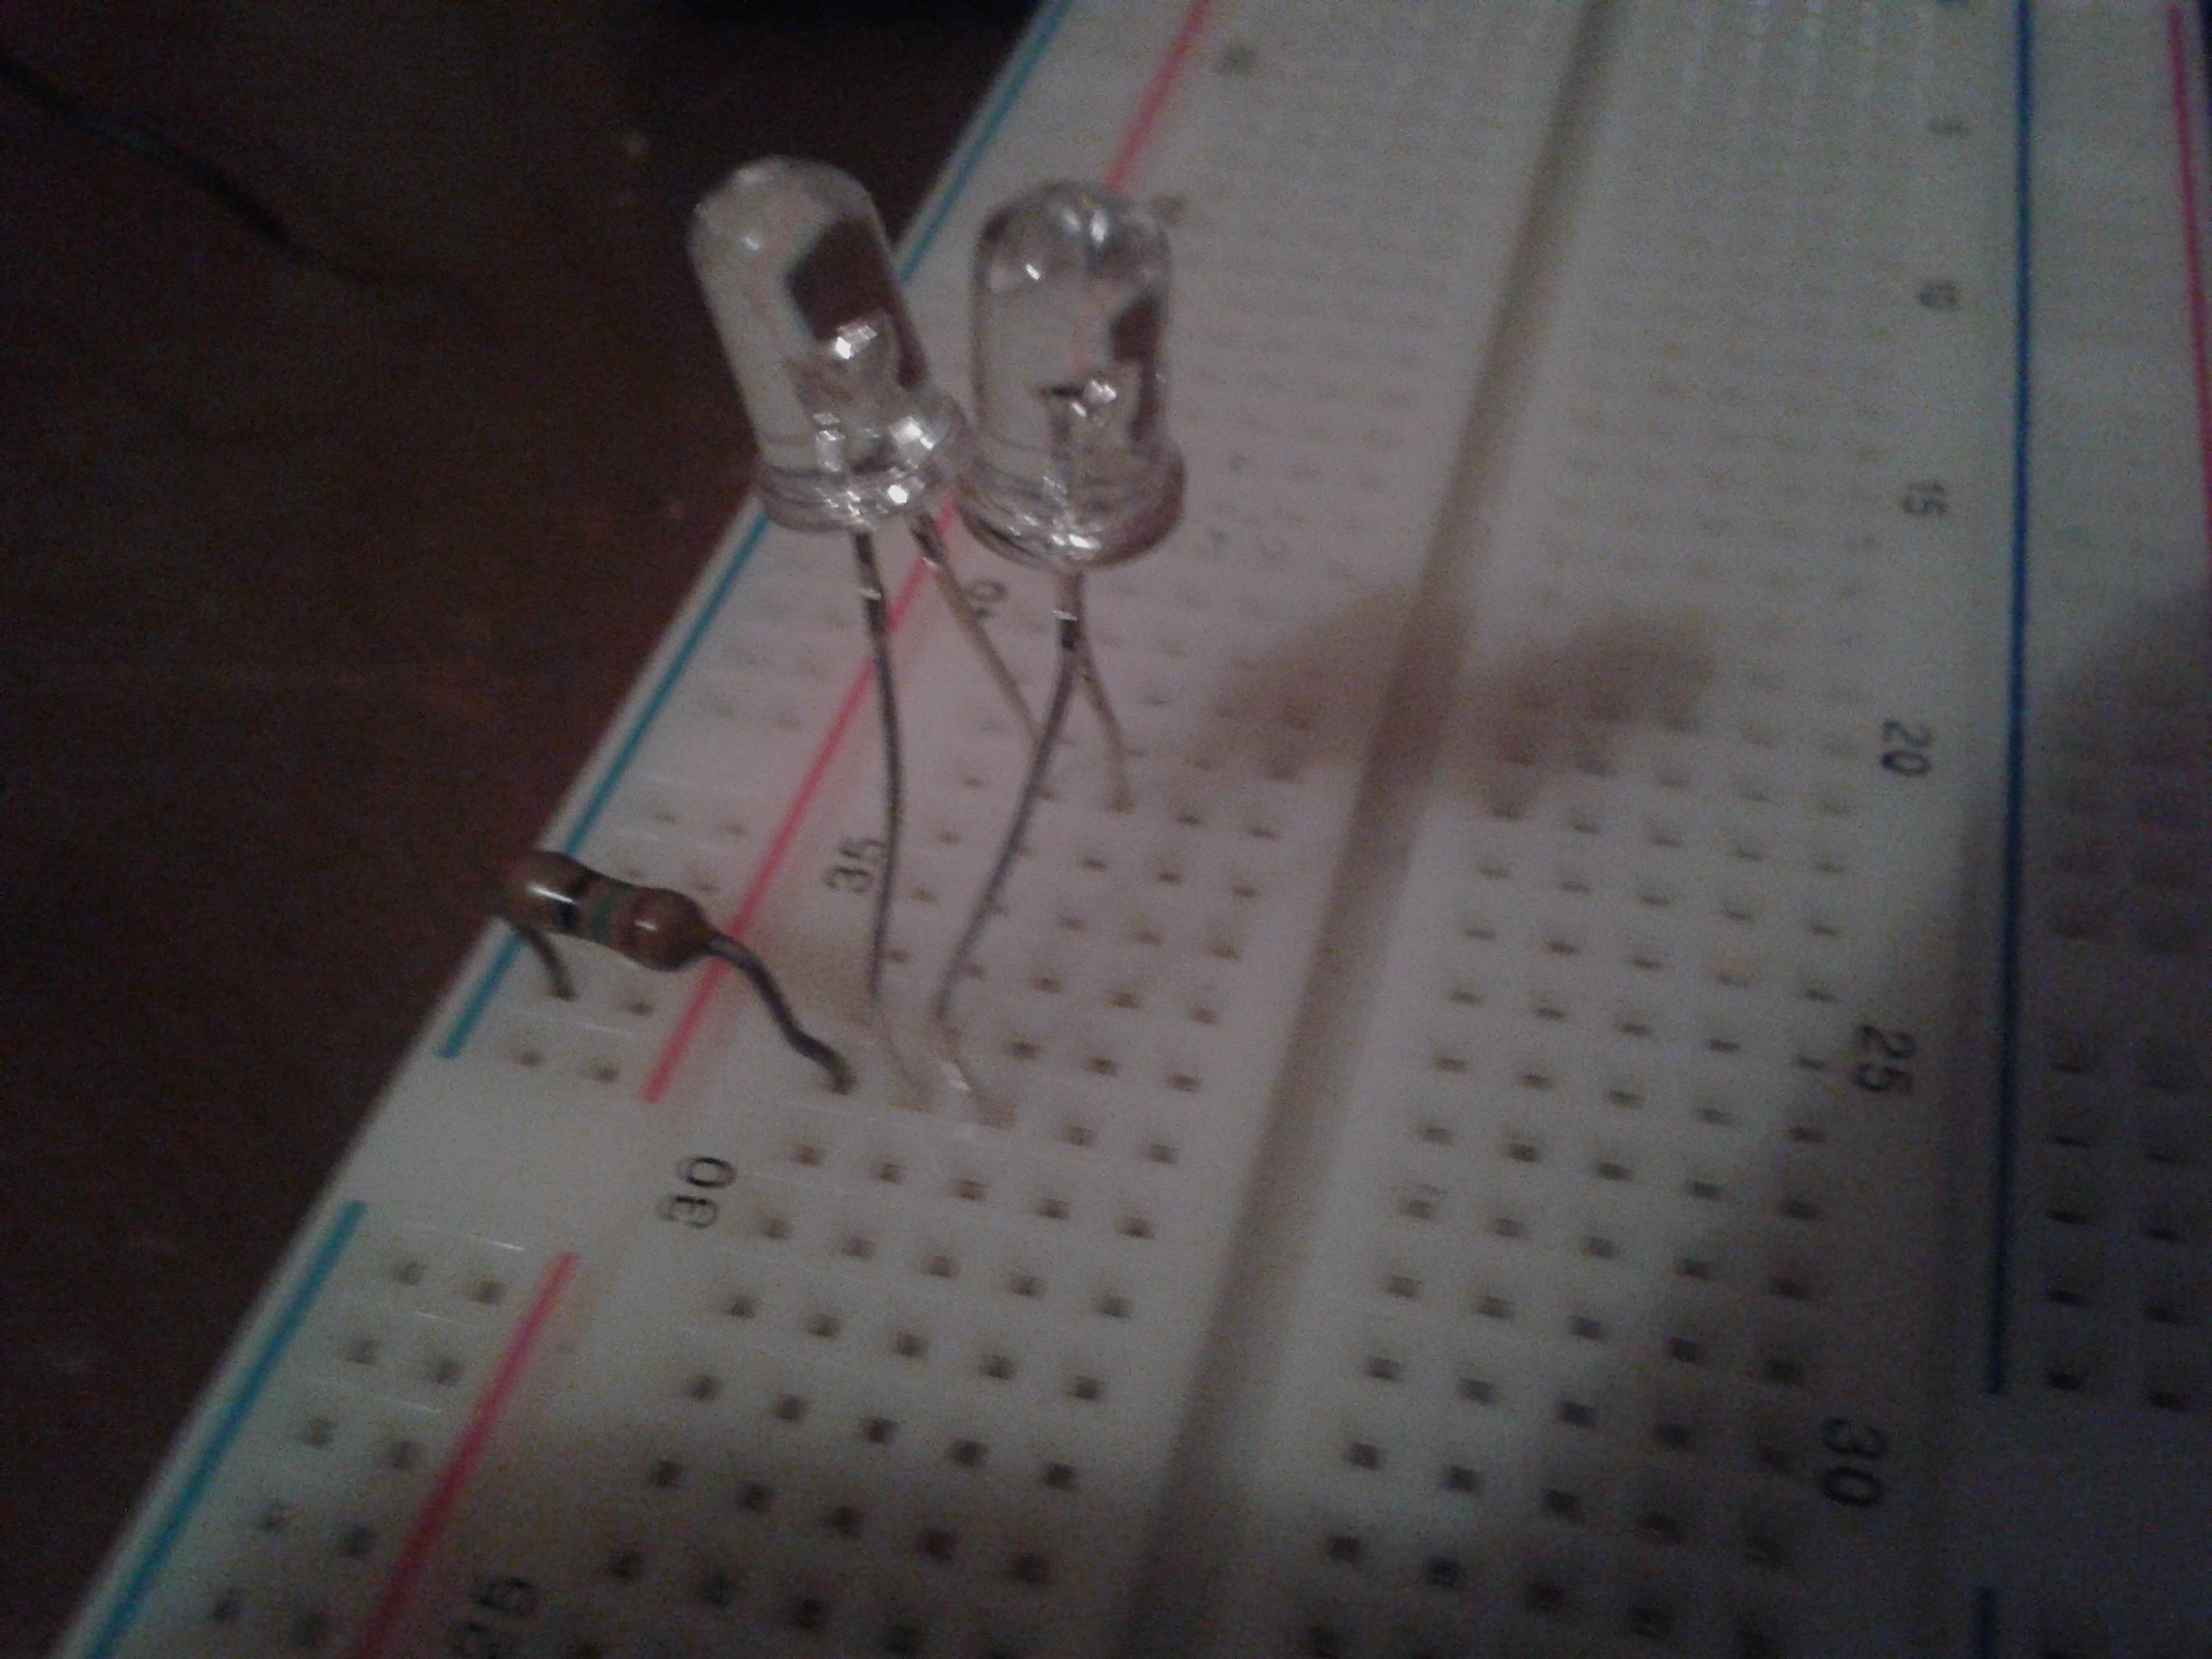
\includegraphics[width=0.4\textwidth,height=0.17\textheight]{mixto}
	\caption{Resistencias en serie y en paralelo simultáneamente.}
\end{figure}

\section{Mediciones con voltímetro}

Para medir voltajes se debe de conectar el multímetro a los extremos de los componentes que se desean medir. La siguiente imagen muestra cómo hacerlo.
\\ 

\begin{figure}[h!]
	\centering
	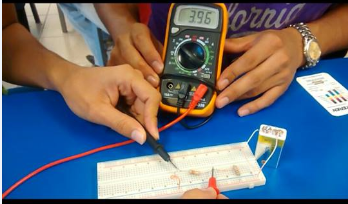
\includegraphics[width=0.6\textwidth,height=0.25\textheight]{voltaje}
	\caption{Medición de voltaje.}
\end{figure}

Análogamente, para medir corrientes el multímetro debe ubicarse en el paso de la corriente que se desea medir, tal como lo ilustra la siguiente figura.
\\ 

\begin{figure}[h!]
	\centering
	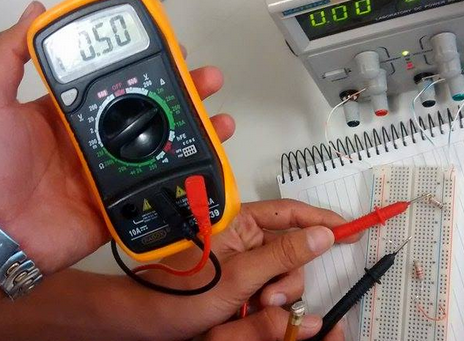
\includegraphics[width=0.6\textwidth,height=0.25\textheight]{corriente}
	\caption{Medición de corriente.}
\end{figure}

\section{Osciloscopio}
Un osciloscopio es un aparato que sirve para medir y visualizar las señales de salida de un circuito. Su interfaz gráfica permite el análisis cualitativo y facilita la toma de diversos datos en la dinámica del circuito estudiado. El osciloscopio que usaremos es de marca Tektronix, de la serie TDS 210. En la siguiente figura se puede apreciar el panel frontal del osciloscopio, el cual se compone de una pantalla y una serie de botones, perillas y entradas cuya función explicaremos más adelante.\\

\begin{figure}[h!]
	\centering
	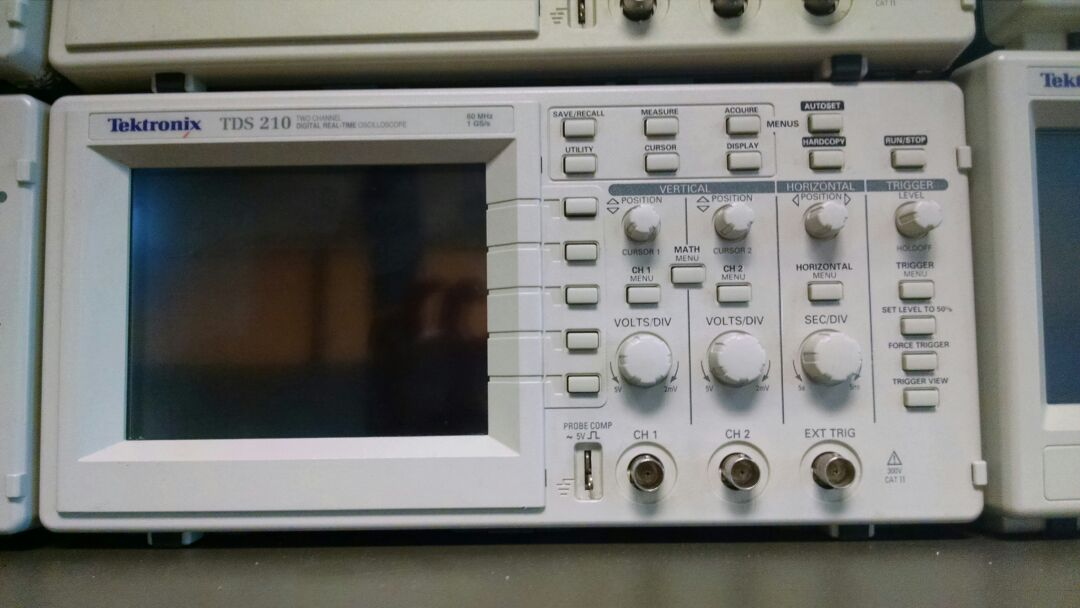
\includegraphics[width=0.6\textwidth,height=0.25\textheight]{osciloscopio.jpg}
	\caption{Osciloscopio TDS 210}
\end{figure}

Los comandos del osciloscopio están organizados por funciones. Los botones cercanos a la pantalla permiten navegar por diversas opciones e interactuar con la interfaz gráfica del osciloscopio. Los botones de la parte superior permiten seleccionar diferentes menús y controlar la señal de entrada. Por otra parte, hay grupos de comandos que permiten mover y modificar los cursores en la pantalla. Estos cursores se usan principalmente para seleccionar un punto específico de la señal en la pantalla. Además de estos, hay un grupo de comandos que sirven para modificar el trigger, el cual permite controlar el muestreo de las señales periódicas. En la siguiente figura se puede apreciar el grupo de controladores verticales del cursor.\\

\begin{figure}[h!]
	\centering
	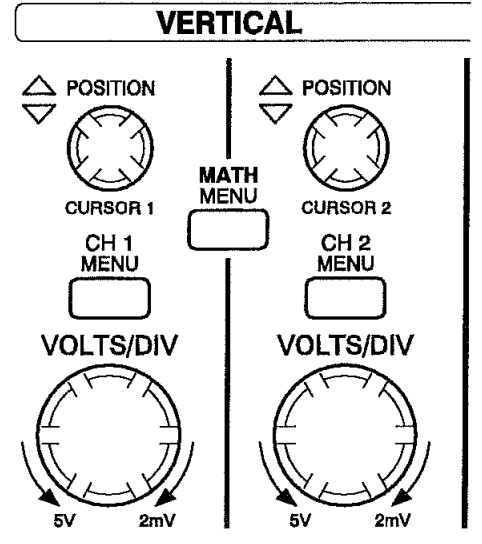
\includegraphics[width=0.3\textwidth,height=0.25\textheight]{Osci-vertical}
	\caption{Controladores verticales de cursor}
\end{figure}

Donde los comandos tienen las siguientes funciones:
\begin{itemize}
	\item \textbf{Position:} Controla la posición vertical del cursor o del canal. 
	\item \textbf{CH Menu:} Muestra el menú de entrada de canal y permite mostrar o quitar la señal de dicho canal.
	\item \textbf{Math Menu:} Muestra el menu de operaciones matemáticas para las señales.
	\item \textbf{Volts/Div:} Permite modificar las escalas en las que se muestran la señal en el eje vertical.

\end{itemize}

En la siguiente figura se muestra por su parte, el grupo de controladores horizontales.

\begin{figure}[h!]
	\centering
	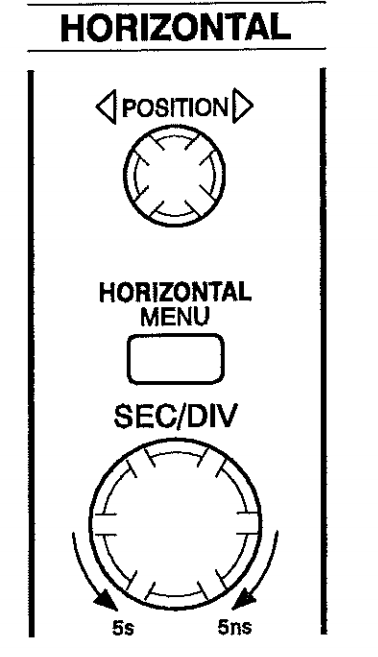
\includegraphics[width=0.3\textwidth,height=0.25\textheight]{osc-horizontal}
	\caption{Controladores horizontales de cursor}
\end{figure}

Donde los comandos tienen las siguientes funciones:
\begin{itemize}
	\item \textbf{Position:} Controla la posición horizontal de todos los canales.
	\item \textbf{Horizontal Menu:} Muestra el menu de medida horizontal.
	\item \textbf{Sec/Div:} Permite modificar las escalas en las que se muestran la señal en el eje horizontal.
\end{itemize}

Los controladores de trigger se muestran en la siguiente figura 10. Allí los comandos tienen las siguientes funciones:

\begin{itemize}
	\item \textbf{Level-Holdoff:} En el modo Level, modifica la amplitud que tiene que cruzar la señal para causar una adquisición. En modo Holdoff, selecciona el tiempo antes de que otro trigger pueda ser aceptado.
	\item \textbf{Trigger Menu:} Muestra el menu de trigger.
	\item \textbf{Set Level to 50\%:} Modifica el nivel del trigger al 50\% del nivel de la señal.
	\item \textbf{Force Trigger:} Empieza la adquisición sin importar si la amplitud de la señal supera el trigger.
	\item \textbf{Trigger View:} Muestra el trigger.
\end{itemize}

\begin{figure}[h!]
	\centering
	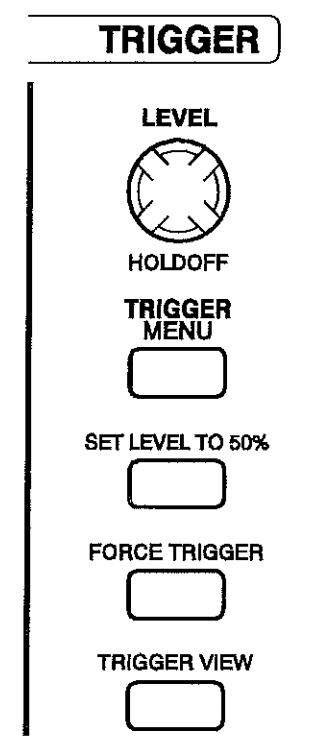
\includegraphics[width=0.20\textwidth,height=0.35\textheight]{osc-trigger}
	\caption{Controladores de trigger}
\end{figure}

En la figura 11 se pueden ver los comandos de control general. \\

\begin{figure}[h!]
	\centering
	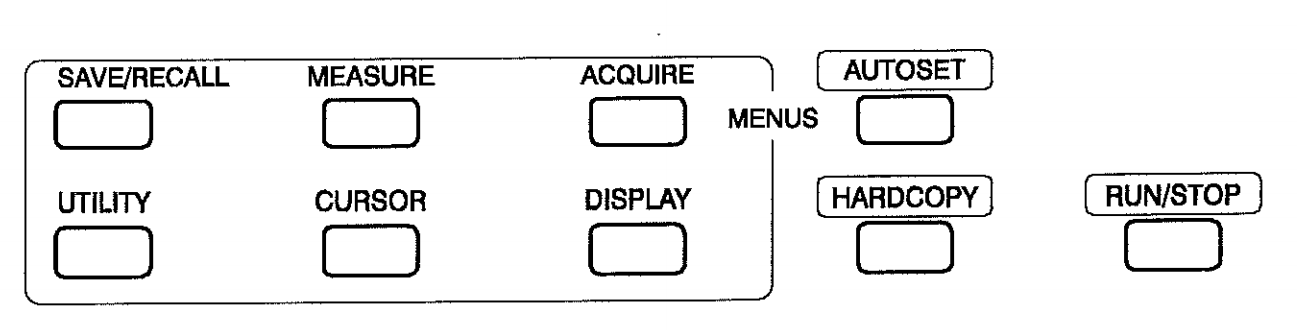
\includegraphics[width=0.60\textwidth,height=0.25\textheight]{osc-control}
	\caption{Controladores generales}
\end{figure}


Estos tienen las siguientes funciones:

\begin{itemize}
	\item \textbf{Save/Recall:} Muestra el menú para salvar y cargar señales.
	\item \textbf{Measure:} Muestra el menú de medidas.
	\item \textbf{Acquire:} Muestra el menú de adquisición de la señal.
	\item \textbf{Cursor:} Muestra el menú de cursores donde se permite controlar qué cursor se mueve con los paneles de comandos horizontales y verticales.
	\item \textbf{Utility:} Muestra el menú de utilidades.
	\item \textbf{Autoset:} Selecciona automáticamente los parámetros para mostrar una señal útil. (No siempre funciona)
	\item \textbf{Hardcopy:} Se usa para imprimir. Necesita una impresora especial conectada al dispositivo.
	\item \textbf{Run/Stop:} Empieza o termina el muestreo.\\
\\
Entre otras opciones la función Measure permite hacer diversas medidas de la señal analizada. En el osciloscopio con el que trabajaremos podremos medir el voltaje rms en un ciclo, el voltaje medio, el voltaje pico-pico, el periodo y la frecuencia de la señal analizada.

\end{itemize}


\section{Generador de señales}
Un generador de señales es una fuente de potencial que permite generar voltajes de forma sinusoidal, cuadrada o triangular. Este dispositivo permite también modificar la frecuencia y la amplitud de estas señales. En el laboratorio utilizaremos un generador marca Tektronix de la serie CFG253. En la siguiente figura se puede ver una fotografía de la parte frontal de dos de estos generadores.\\

\begin{figure}[h!]
	\centering
	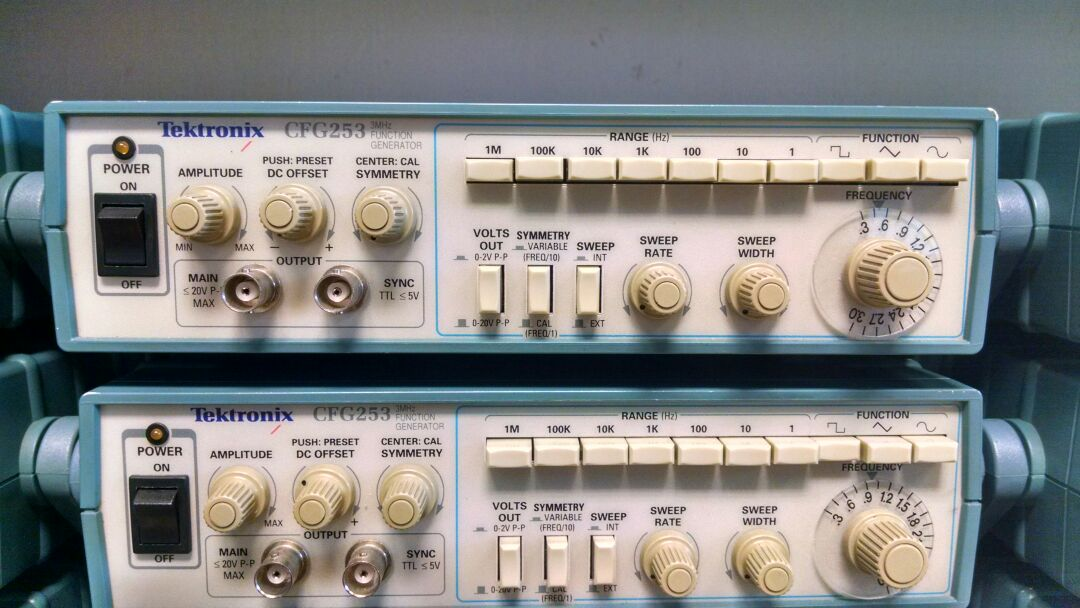
\includegraphics[width=0.60\textwidth,height=0.25\textheight]{generador}
	\caption{Generador de señales}
\end{figure}

En la figura 13 se ve un diagrama claro de los comandos de este dispositivo. Aquí las funciones son las siguientes:

\begin{itemize}
	\item \textbf{1:} Muestra si el dispositivo está encendido o apagado.
	\item \textbf{2:} Determina la amplitud de la señal que sale por el cable principal (main).
	\item \textbf{3:} Sirve para controlar la aplitud DC de la señal y su polaridad.
	\item \textbf{4:} Controla la simetría vertical de la señal generada.
	\item \textbf{5:} Determina el rango en que se va a modificar la frecuencia de la señal que sale por el cable principal.
	\item \textbf{6:} Selecciona la forma de la onda de salida: sinusoidal, cuadrada o triangular.
	\item \textbf{7:} Modifica la frecuencia en el rango determindo por (5).
	\item \textbf{8:} Ajusta la amplitud de barrido de la señal.
	\item \textbf{9:} Ajusta la frecuencia del generador de barrido interno.
	\item \textbf{10:} Activa las opciones (8) y (9).
	\item \textbf{11:} Divide la frecuencia de la señal de salida por 10 y permite ajustar la simetría de la señal con (4).
	\item \textbf{12:} Permite variar el rango en el que se controla la amplitud del voltaje pico-pico de la señal.

\begin{figure}[h!]
	\centering
	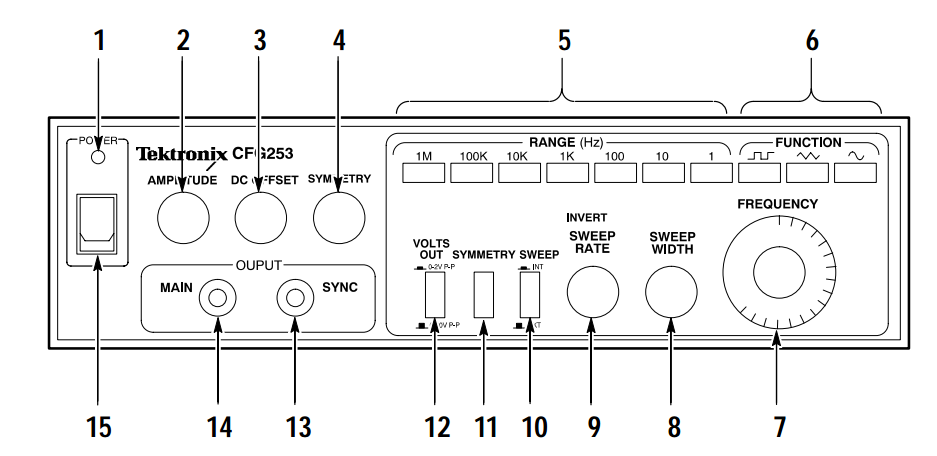
\includegraphics[width=0.60\textwidth,height=0.25\textheight]{Generador-Funciones}
	\caption{Generador de señales - Comandos}
\end{figure}




\end{itemize}
	
	
\end{document}








